% Szablony LaTeX dla zestawień ewolucji wymiaru dla różnych metod normalizacji

\begin{figure}[htbp]
    \centering
    \begin{subfigure}[b]{0.48\textwidth}
        \centering
        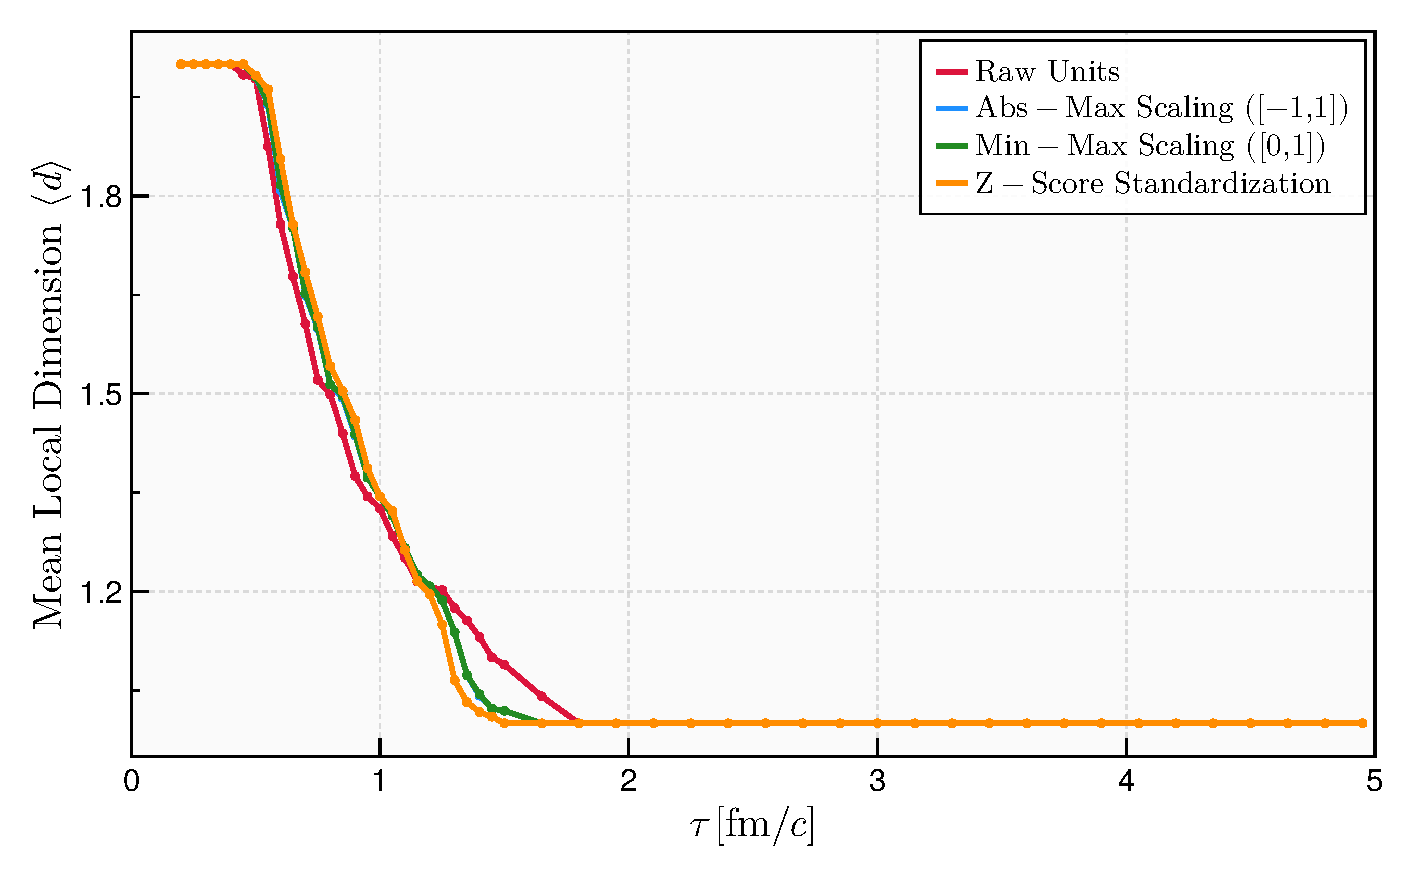
\includegraphics[width=\linewidth]{best_practices_lpca/mean_dimension_vs_tau_mis_dims.pdf}
        \caption{MIS: \emph{dims} ($k=24$)}
        \label{fig:mean_dim_mis_dims}
    \end{subfigure}
    \hfill
    \begin{subfigure}[b]{0.48\textwidth}
        \centering
        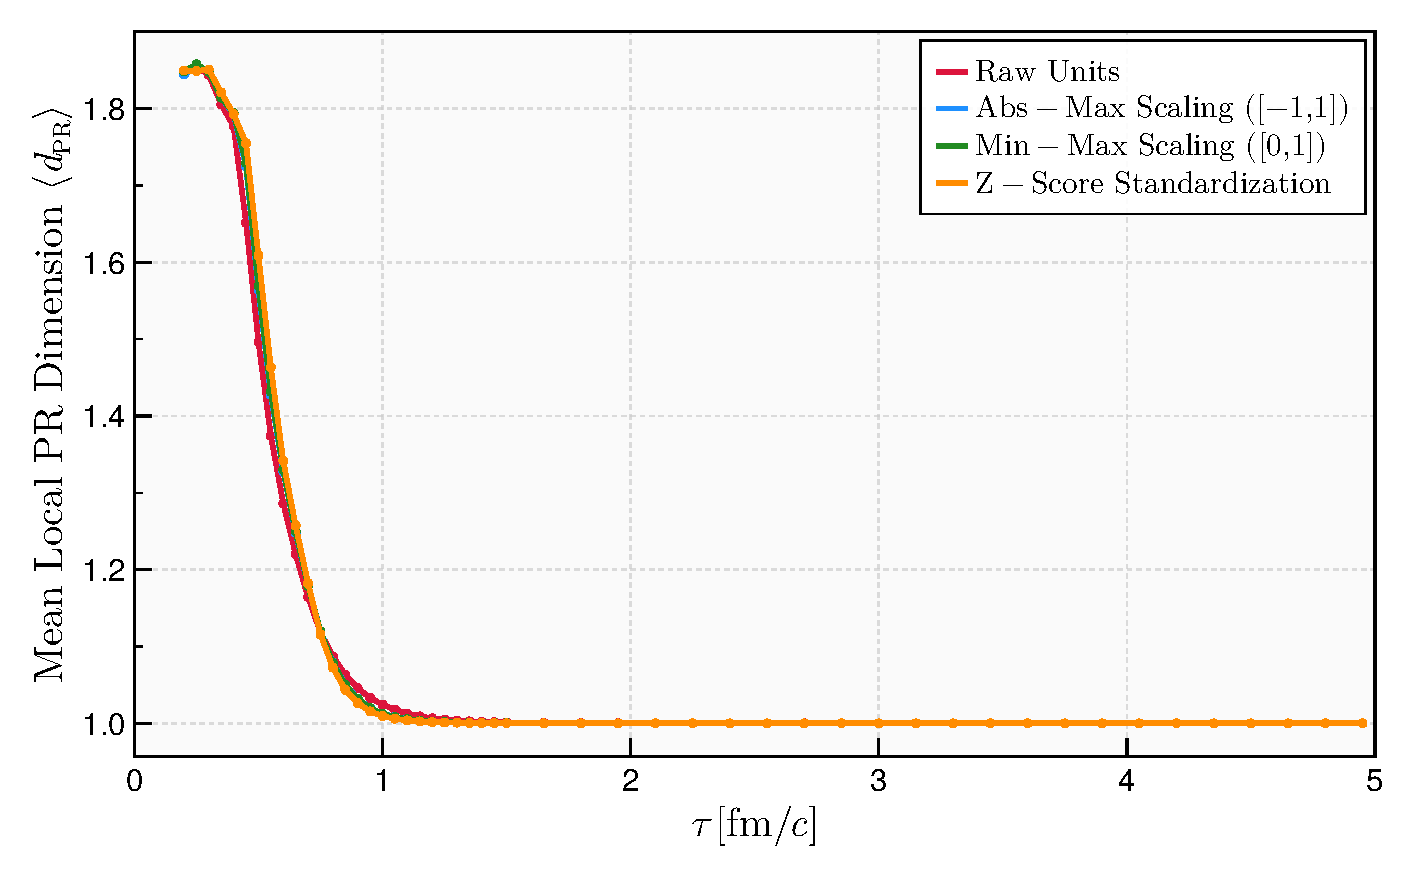
\includegraphics[width=\linewidth]{best_practices_lpca/mean_dimension_vs_tau_mis_pr.pdf}
        \caption{MIS: \emph{pr} ($k=24$)}
        \label{fig:mean_dim_mis_pr}
    \end{subfigure}

    \vspace{0.8em}

    \begin{subfigure}[b]{0.48\textwidth}
        \centering
        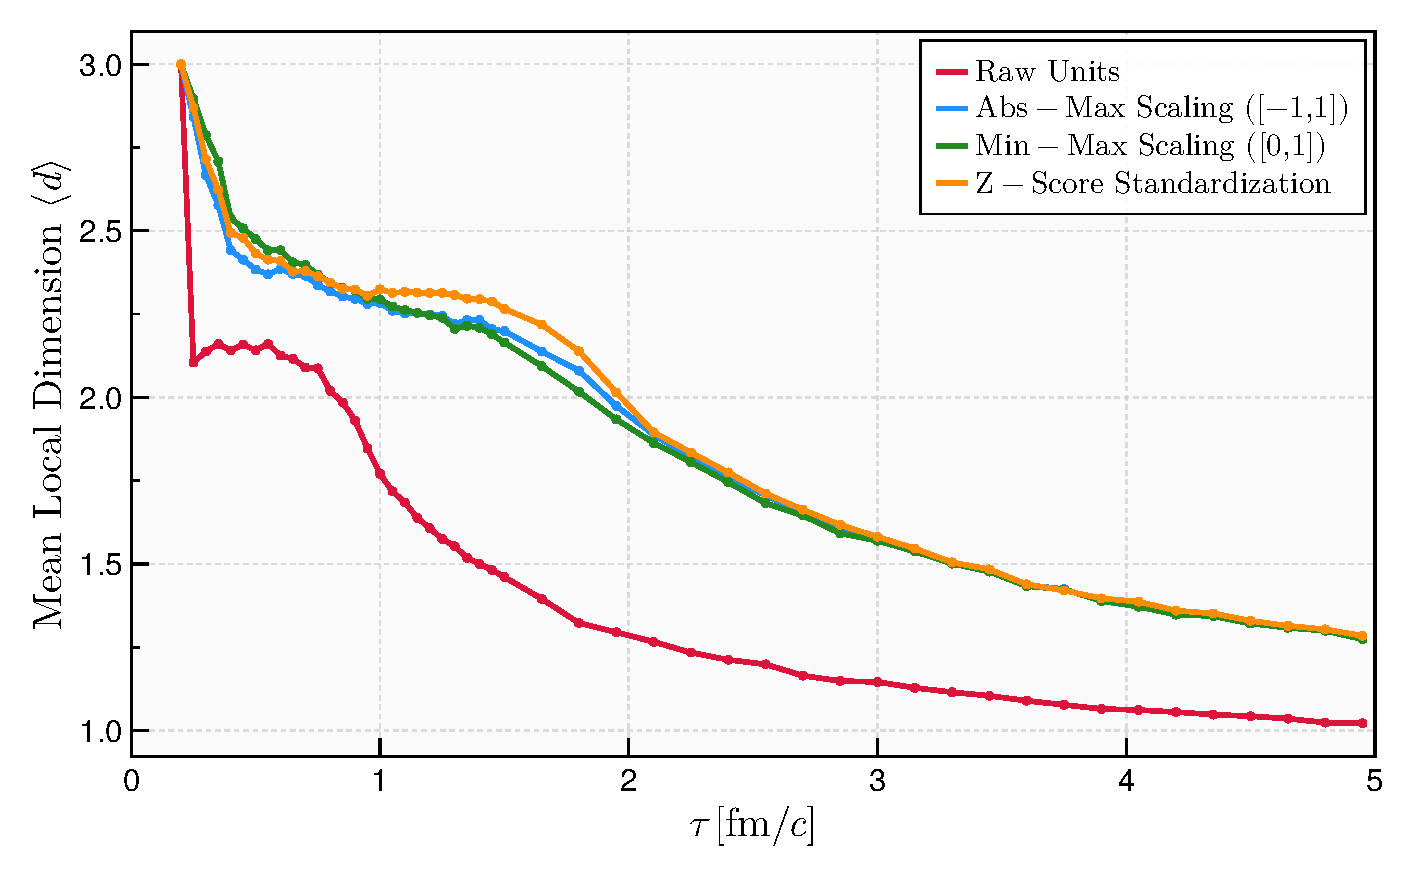
\includegraphics[width=\linewidth]{best_practices_lpca/mean_dimension_vs_tau_hjsw_dims.pdf}
        \caption{HJSW: \emph{dims} ($k=24$)}
        \label{fig:mean_dim_hjsw_dims}
    \end{subfigure}
    \hfill
    \begin{subfigure}[b]{0.48\textwidth}
        \centering
        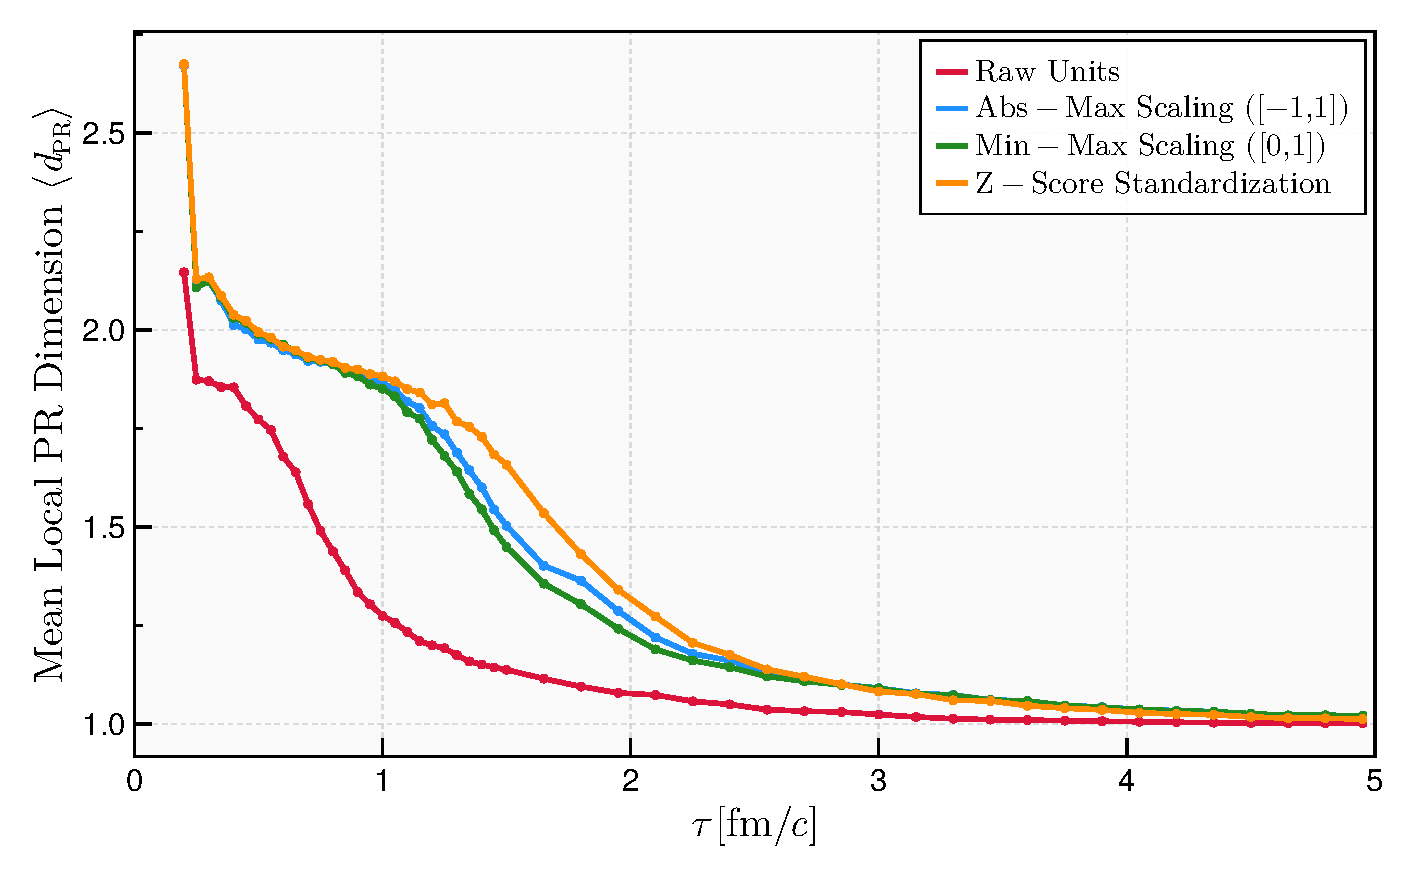
\includegraphics[width=\linewidth]{best_practices_lpca/mean_dimension_vs_tau_hjsw_pr.pdf}
        \caption{HJSW: \emph{pr} ($k=24$)}
        \label{fig:mean_dim_hjsw_pr}
    \end{subfigure}

    \caption{Porównanie wrażliwości metod normalizacji przestrzeni fazowej w czasie $\tau \in [0.20, 5.00]\,\mathrm{fm}/c$ dla ustalonej liczby sąsiadów $k=24$. Brak standaryzacji (Raw Units, linia czerwona) powoduje pozorny kolaps wymiaru z powodu rozbieżności skal fizycznych, podczas gdy standaryzacje Z-Score, Abs-Max i Min-Max poprawnie identyfikują strukturę wielowymiarową.}
    \label{fig:mean_dimension_all_methods_comparison}
\end{figure}
